\section{Multiplications de matrices}\label{sec:matrixmultiplication}

Les programmes font une multiplication de matrice tel que:

\[
A = \begin{bmatrix} 
    a_{11} & a_{12} & \dots & a_{1n}\\
    \vdots & \ddots &  \\
    a_{m1} &        & & a_{mn} 
    \end{bmatrix}
    ,
B = \begin{bmatrix} 
    b_{11} & b_{12} & \dots & b_{1p}\\
    \vdots & \ddots &  \\
    b_{n1} &        & & b_{np} 
    \end{bmatrix}
    ,
C = \begin{bmatrix} 
    c_{11} & c_{12} & \dots & c_{1p}\\
    \vdots & \ddots &  \\
    c_{m1} &        &  & c_{mp} 
    \end{bmatrix}
    ;
    AB = C
\]

Les programmes génèrent ainsi des tableaux de une dimension de tailles 
$A_{lignes} \quad * \quad A_{colonnes}$ et $B_{lignes} \quad * \quad B_{colonnes}$
avec des nombres aléatoires pour $A$ et $B$ respectivement, 
et une taille $A_{lignes} \quad * \quad B_{colonnes}$ avec des zéros pour $C$ avant 
de réaliser la multiplication.

On s'assure aussi avant de commencer tout traitement que $A_{colonnes} = B_{lignes}$.

\subsection{Implémentation naïve}  

\subsubsection{Idée de l'implémentation}

Pour l'implémentation naïve, on s'est basé sur la formule mathématique suivante:
\[
    C_{ij} = \sum_{k=1}^{n} a_{ik}b_{kj}\quad\textrm{pour}\quad i = 1, \dots, m\quad \textrm{et}\quad j = 1,\dots,p
\]

Cette formule se traduit facilement en \texttt{OpenCL} en calculant chaque $C_{ij}$ dans un \textit{work item}. 
On obtient ainsi le kernel suivant:

\begin{lstlisting}[language=c]
__kernel void matrix_mult(__global float *a,
                          __global float* b,
                          __global float* c,
                          const unsigned int a_ncol,
                          const unsigned int b_ncol) {
    int rows = get_global_id(0);    /* iterate over rows */
    int columns = get_global_id(1); /* then iterate over columns */

    /* compute value */
    float value = 0;
    for (unsigned int i = 0 ; i < a_ncol ; i++) {
        value += a[rows * a_ncol + i] * b[i * b_ncol + columns];
    }

    c[rows * b_ncol + columns] = value;
}
\end{lstlisting}    
\vspace{20pt}

Comme on peut le remarquer, on ne passe pas de matrices en tant que tel. En effet 
comme mentionné dans la Section~\ref{sec:memory_model}, les \textit{buffers} sont 
forcément des vecteurs. On peut ici voir que l'on passe la matrice $A$ via le 
premier argument et ainsi les matrices $B$ et $C$. On doit aussi passer la taille 
des colonnes de $A$ et $B$ ici appelées $a\_ncol$ et $b\_ncol$ afin de pouvoir 
parcourir les matrices mises à plats.

En partant du principe que l'ensemble des éléments pour \texttt{OpenCL} ont été 
définis (voir Section~\ref{sec:pyopencl}) et le programme compilé dans la variable 
$program$, la mise oeuvre est réalisée de la façon suivante en \texttt{Python}:
\begin{lstlisting}[language=python]
import numpy as np
import pyopencl as cl

# a_dim is a tuple with (row, column) for A
A = np.random.rand(A_dim[0] * A_dim[1]).astype(np.float32)   
# b_dim ditto
B = np.random.rand(B_dim[0] * B_dim[1]).astype(np.float32)   
C = np.zeros(A_dim[1] * B_dim[0], dtype=np.float32)

A_buffer = cl.Buffer(context, flags=cl.mem_flags.READ_ONLY, size=A.nbytes)
B_buffer = cl.Buffer(context, flags=cl.mem_flags.READ_ONLY, size=B.nbytes)
C_buffer = cl.Buffer(context, flags=cl.mem_flags.WRITE_ONLY, size=C.nbytes)

cl.enqueue_copy(queue, src=A, dest=A_buffer)
cl.enqueue_copy(queue, src=B, dest=B_buffer)

kernel_arguments = (A_buffer, B_buffer, C_buffer, A_dim[1], B_dim[1])
# .wait() to wait for the event to finish
program.matrix_mult(queue, 
                   [A_dim[0], B_dim[1]],     # global dimensions
                   None, 
                   *kernel_arguments).wait()

cl.enqueue_copy(queue, src=C_buffer, dest=C)
\end{lstlisting}
\vspace{20pt}

Comme on peut le voir, les \textit{work items} sont crées à partir d'un 
\textit{global NDRange} de deux dimensions correspondant à celles de la 
matrice C. On peut aussi noter qu'on ne fait pas usage de la mémoire locale 
le \textit{local NDRange} étant mis à \textit{None}.

\subsubsection{Résultats}

On a fait trois genres de mesures afin de voir l'éfficacité et la fiabilité 
de l'implémentation: la copie des \textit{buffers}, le temps d'exécution et 
la précision des résultats. Pour faire ces mesures on a exécuté le programme 
pour des matrices carrées de même dimension allant de 10 à 1 500 lignes/colonnes par pas de 10. 
Tous les graphes peuvent êtres retrouvées avec une meilleure résolution en annexe.

\begin{figure}[H]
\begin{center}
    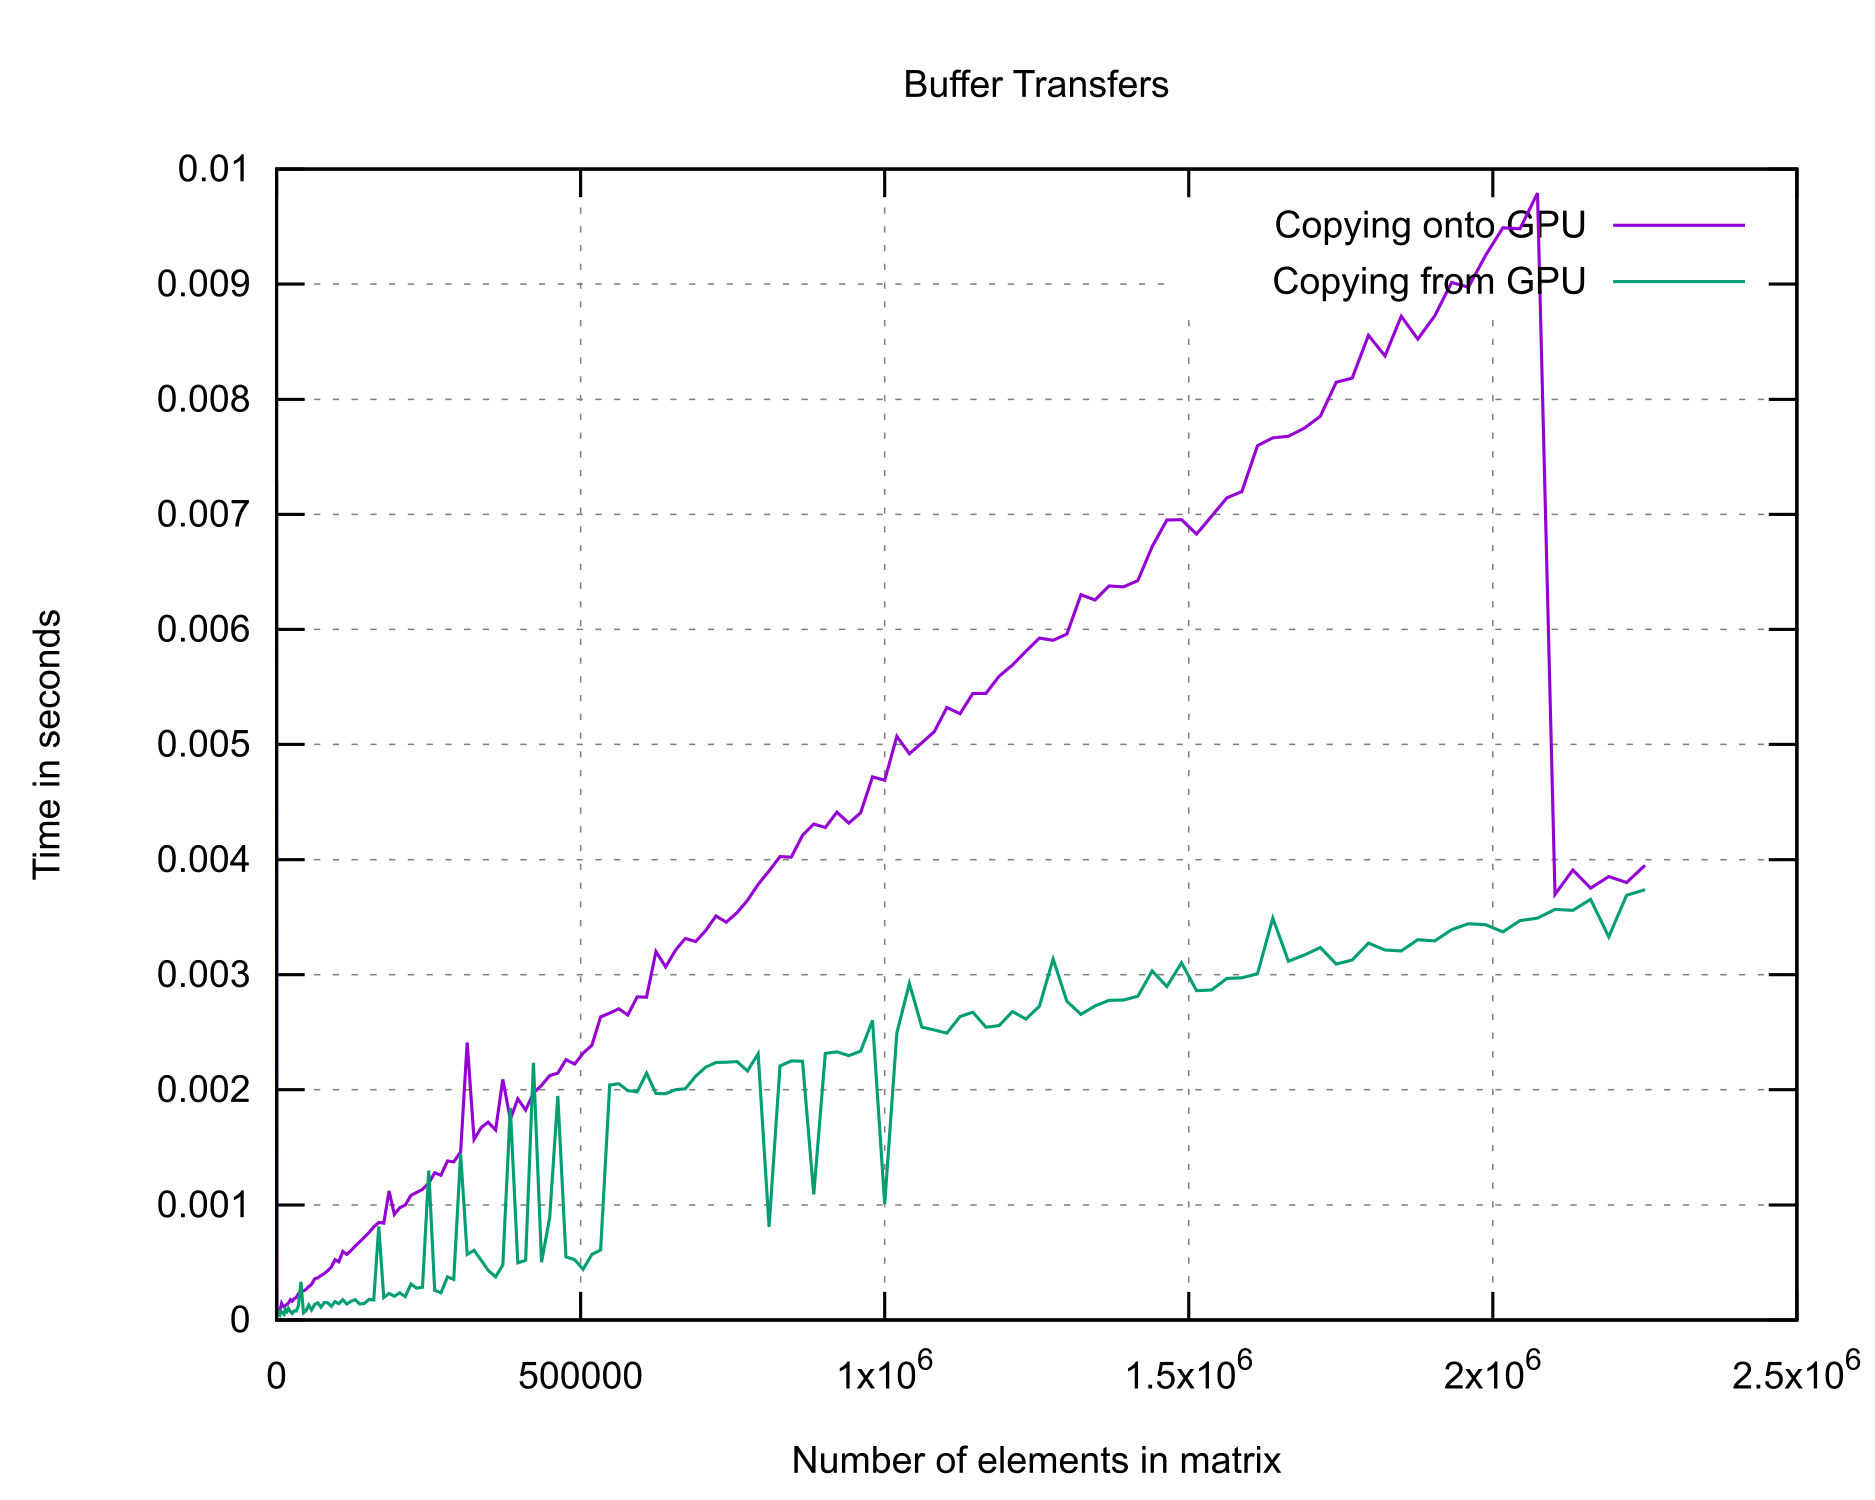
\includegraphics[width=0.6\textwidth]{../../resources/matrix_naive_buffer_transfer.png}
    \caption{Temps de copie des \textit{buffers} de \textit{float32} entre l'hôte et le GPU}
    \label{fig:buffer_transfer_naive}
\end{center}
\end{figure}

La copie des buffers est linéaire comme on peut le voir
(Figure~\ref{fig:buffer_transfer_naive}). Cependant, on constate un gain en 
temps considérable lors de la copie de \textit{A\_buffer} et \textit{B\_buffer}. 
On n'explique pas pourquoi ce gain de temps arrive à ce moment précis cependant 
on en déduit que des optimisations sont faites lorsque le nombre d'élément 
transféré devient considérable. Ici le dernier transfer vers le GPU est de 
4 500 000 éléments soit 144 000 000 bits.

\begin{figure}[H]
\begin{center}
    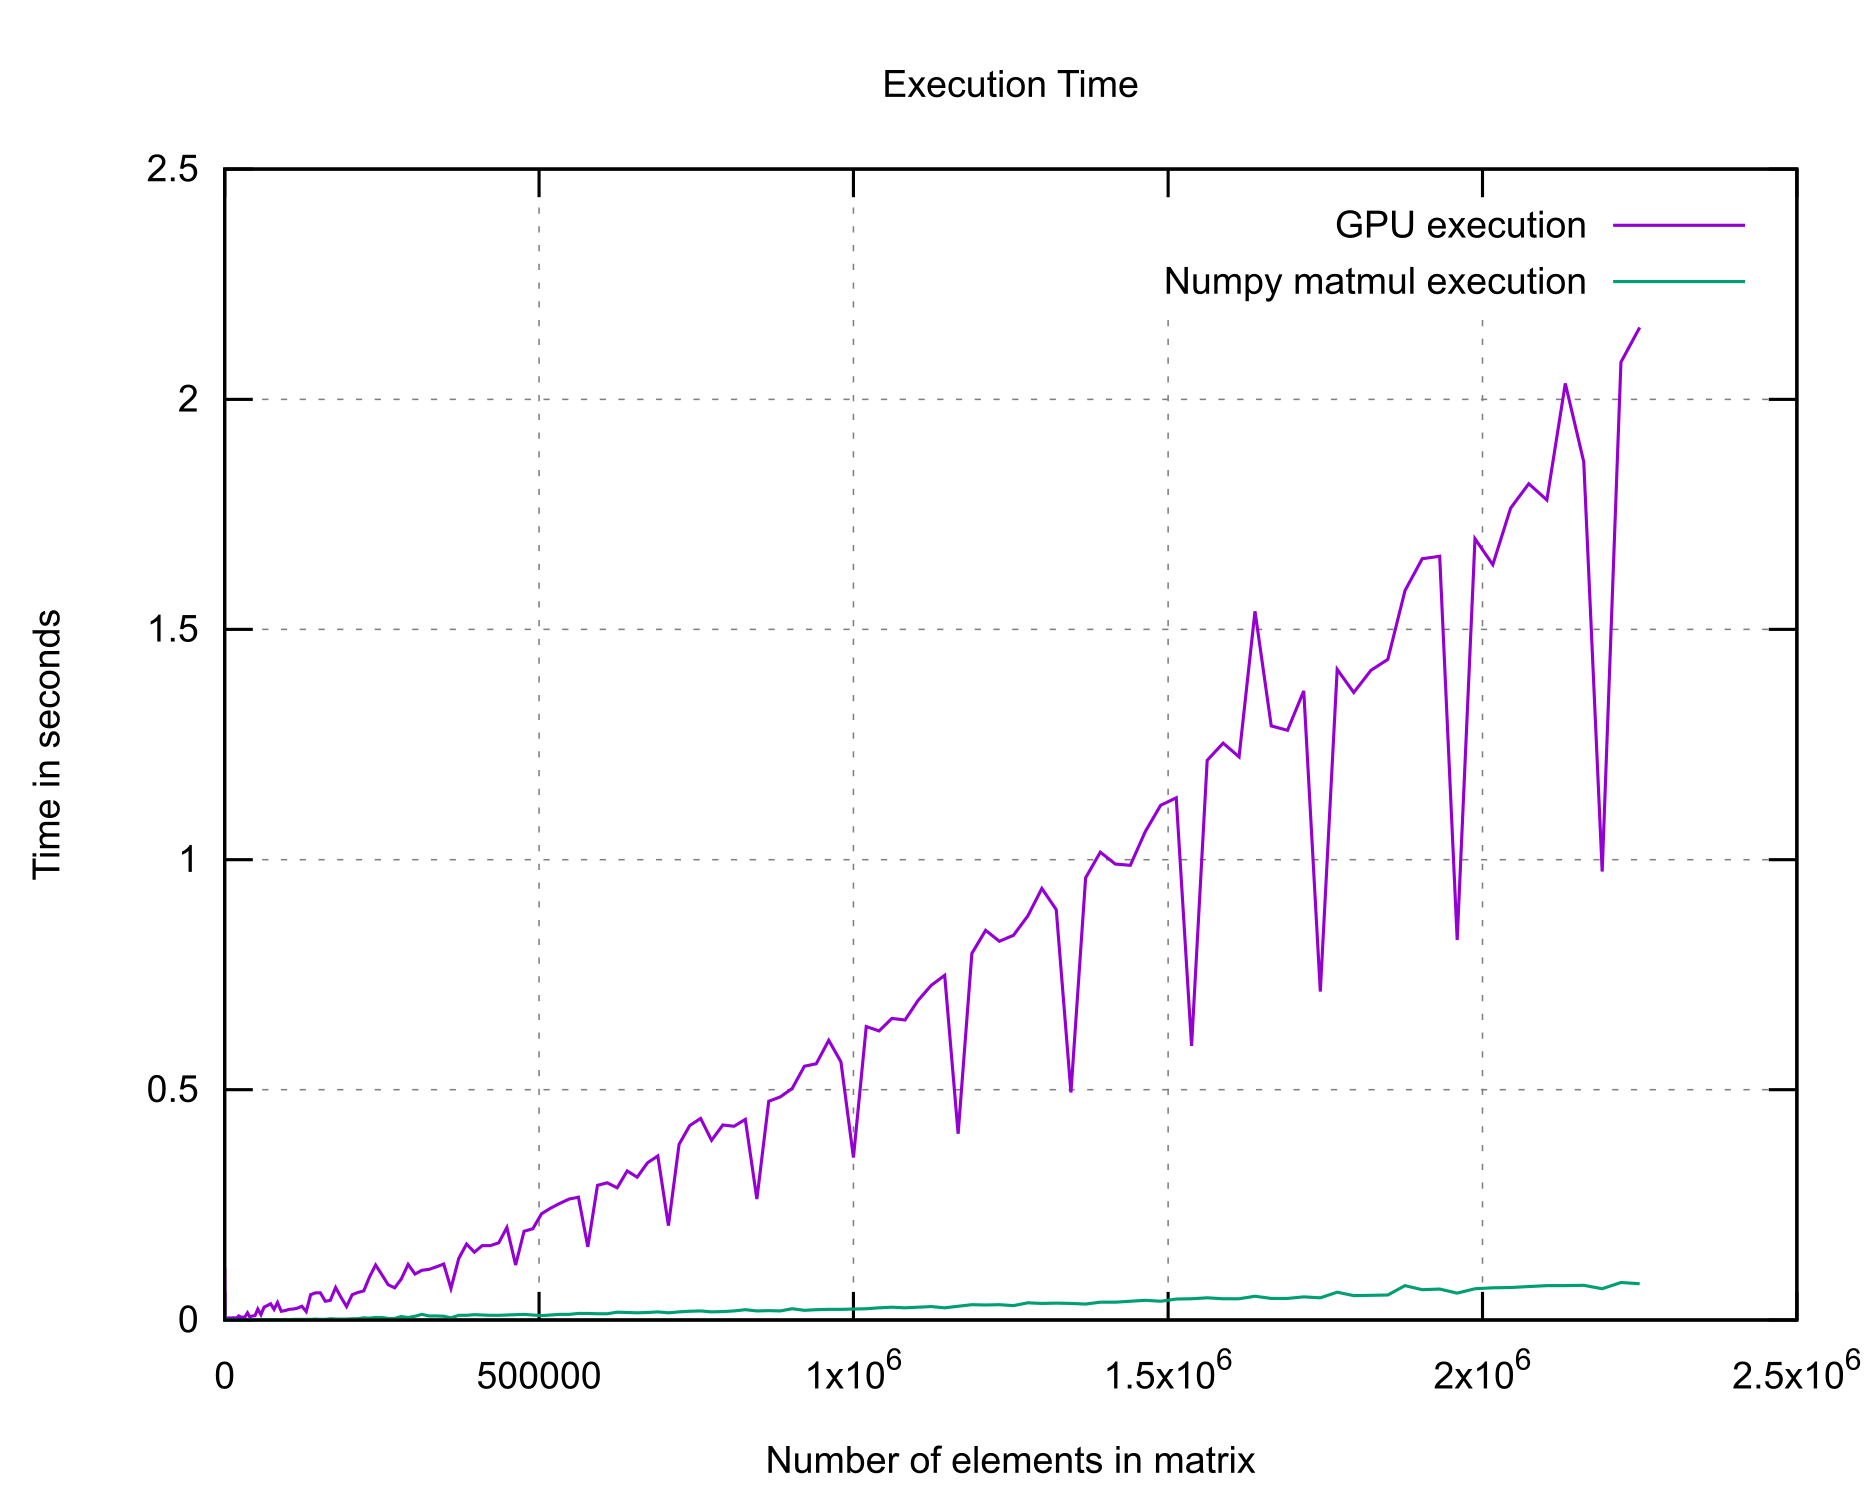
\includegraphics[width=0.6\textwidth]{../../resources/matrix_naive_execution_time.png}
    \caption{Temps d'exécution de notre implémentation et de la méthode Matmult de \texttt{Numpy}
    pour une multiplication sur des \textit{float32}}
    \label{fig:execution_time_naive}
\end{center}
\end{figure}

Le temps d'exécution de notre implémentation est comme attendu en $O(n^3)$ 
(Figure~\ref{fig:execution_time_naive}). On note cependant 
qu'elle est beaucoup plus lente que celle de \texttt{Numpy}. Cela s'explique 
par le fait que tous les \textit{work items} appertenant au même groupe, ils sont tous concurrents. 
De plus, on crée de la contention sur la mémoire global car on a autant de \textit{work items} que 
d'éléments de la matrice $C$ qui tente d'accéder concurrement à la mémoire globale. On remarque 
aussi des gains de performance réguliers qu'on n'explique pas non plus.

\begin{figure}[H]
\begin{center}
    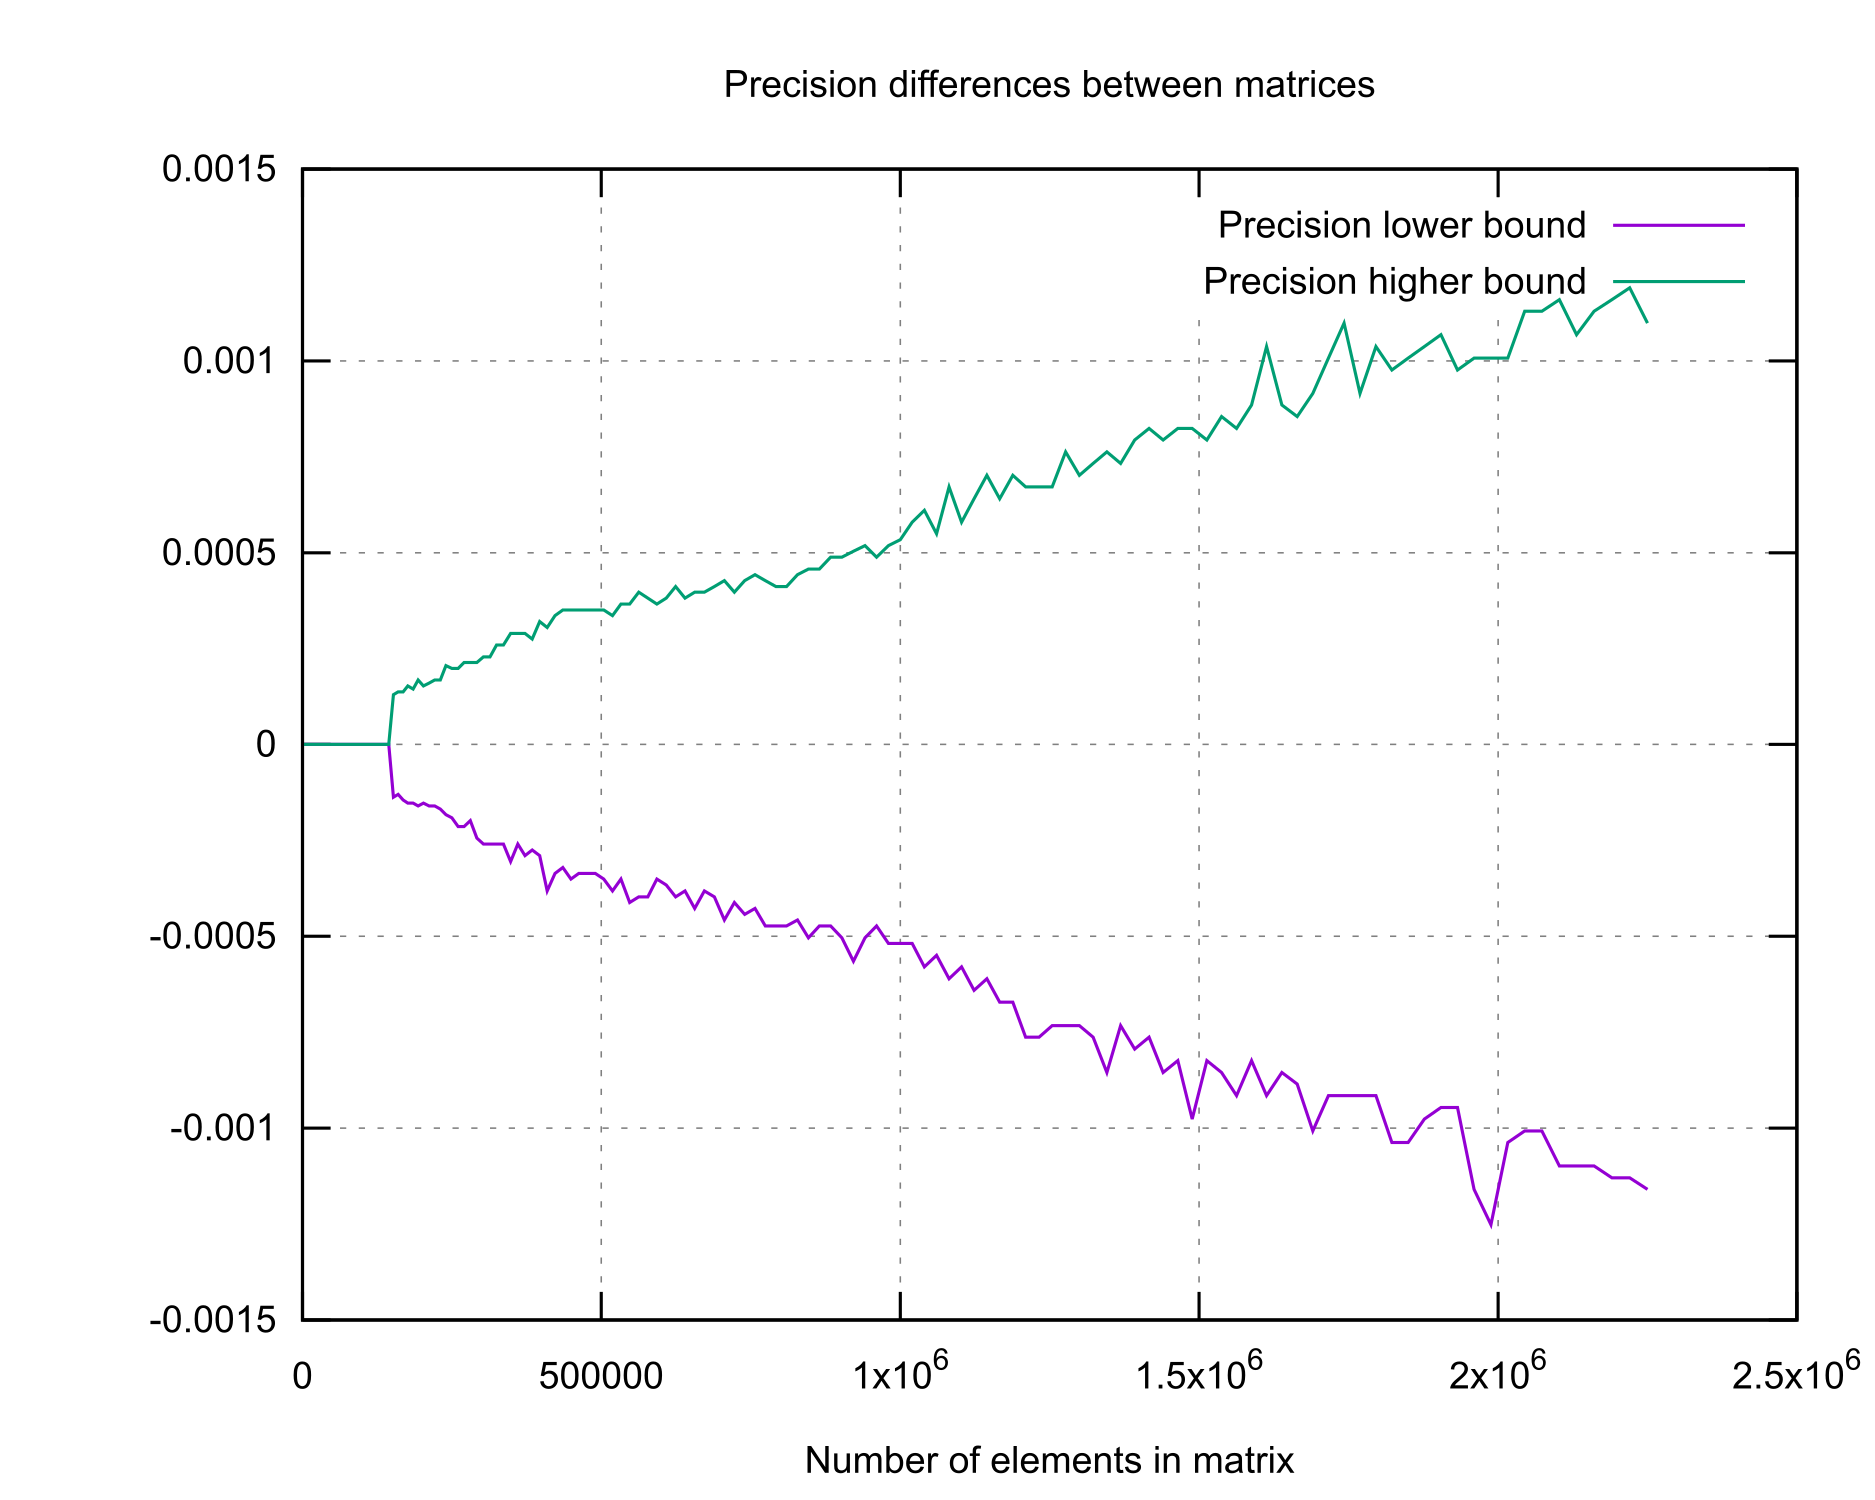
\includegraphics[width=0.6\textwidth]{../../resources/matrix_naive_float_precision.png}
    \caption{Écart de précision existant entre les résultats de la méthode Matmult de Numpy 
    et de notre implémentation pour une multiplication sur des \textit{float32}}
    \label{fig:accuracy_naive}
\end{center}
\end{figure}

Enfin, on constate un écart entre les éléments des matrices résultantes de \texttt{Numpy} et 
de notre implémentation (Figure~\ref{fig:accuracy_naive}). C'est une problématique de calcul 
sur les flottants\footnote{On ne sait pas lequel est le plus précis, la conversion en type \textit{Decimal} 
de \texttt{Python} étant très contraignante}. On peut voir sur la Figure~\ref{fig:accuracy_naive_integers} pour lequel
le calcul a été éffectué sur des entiers que nous n'avons pas d'écarts.

\begin{figure}[H]
\begin{center}
    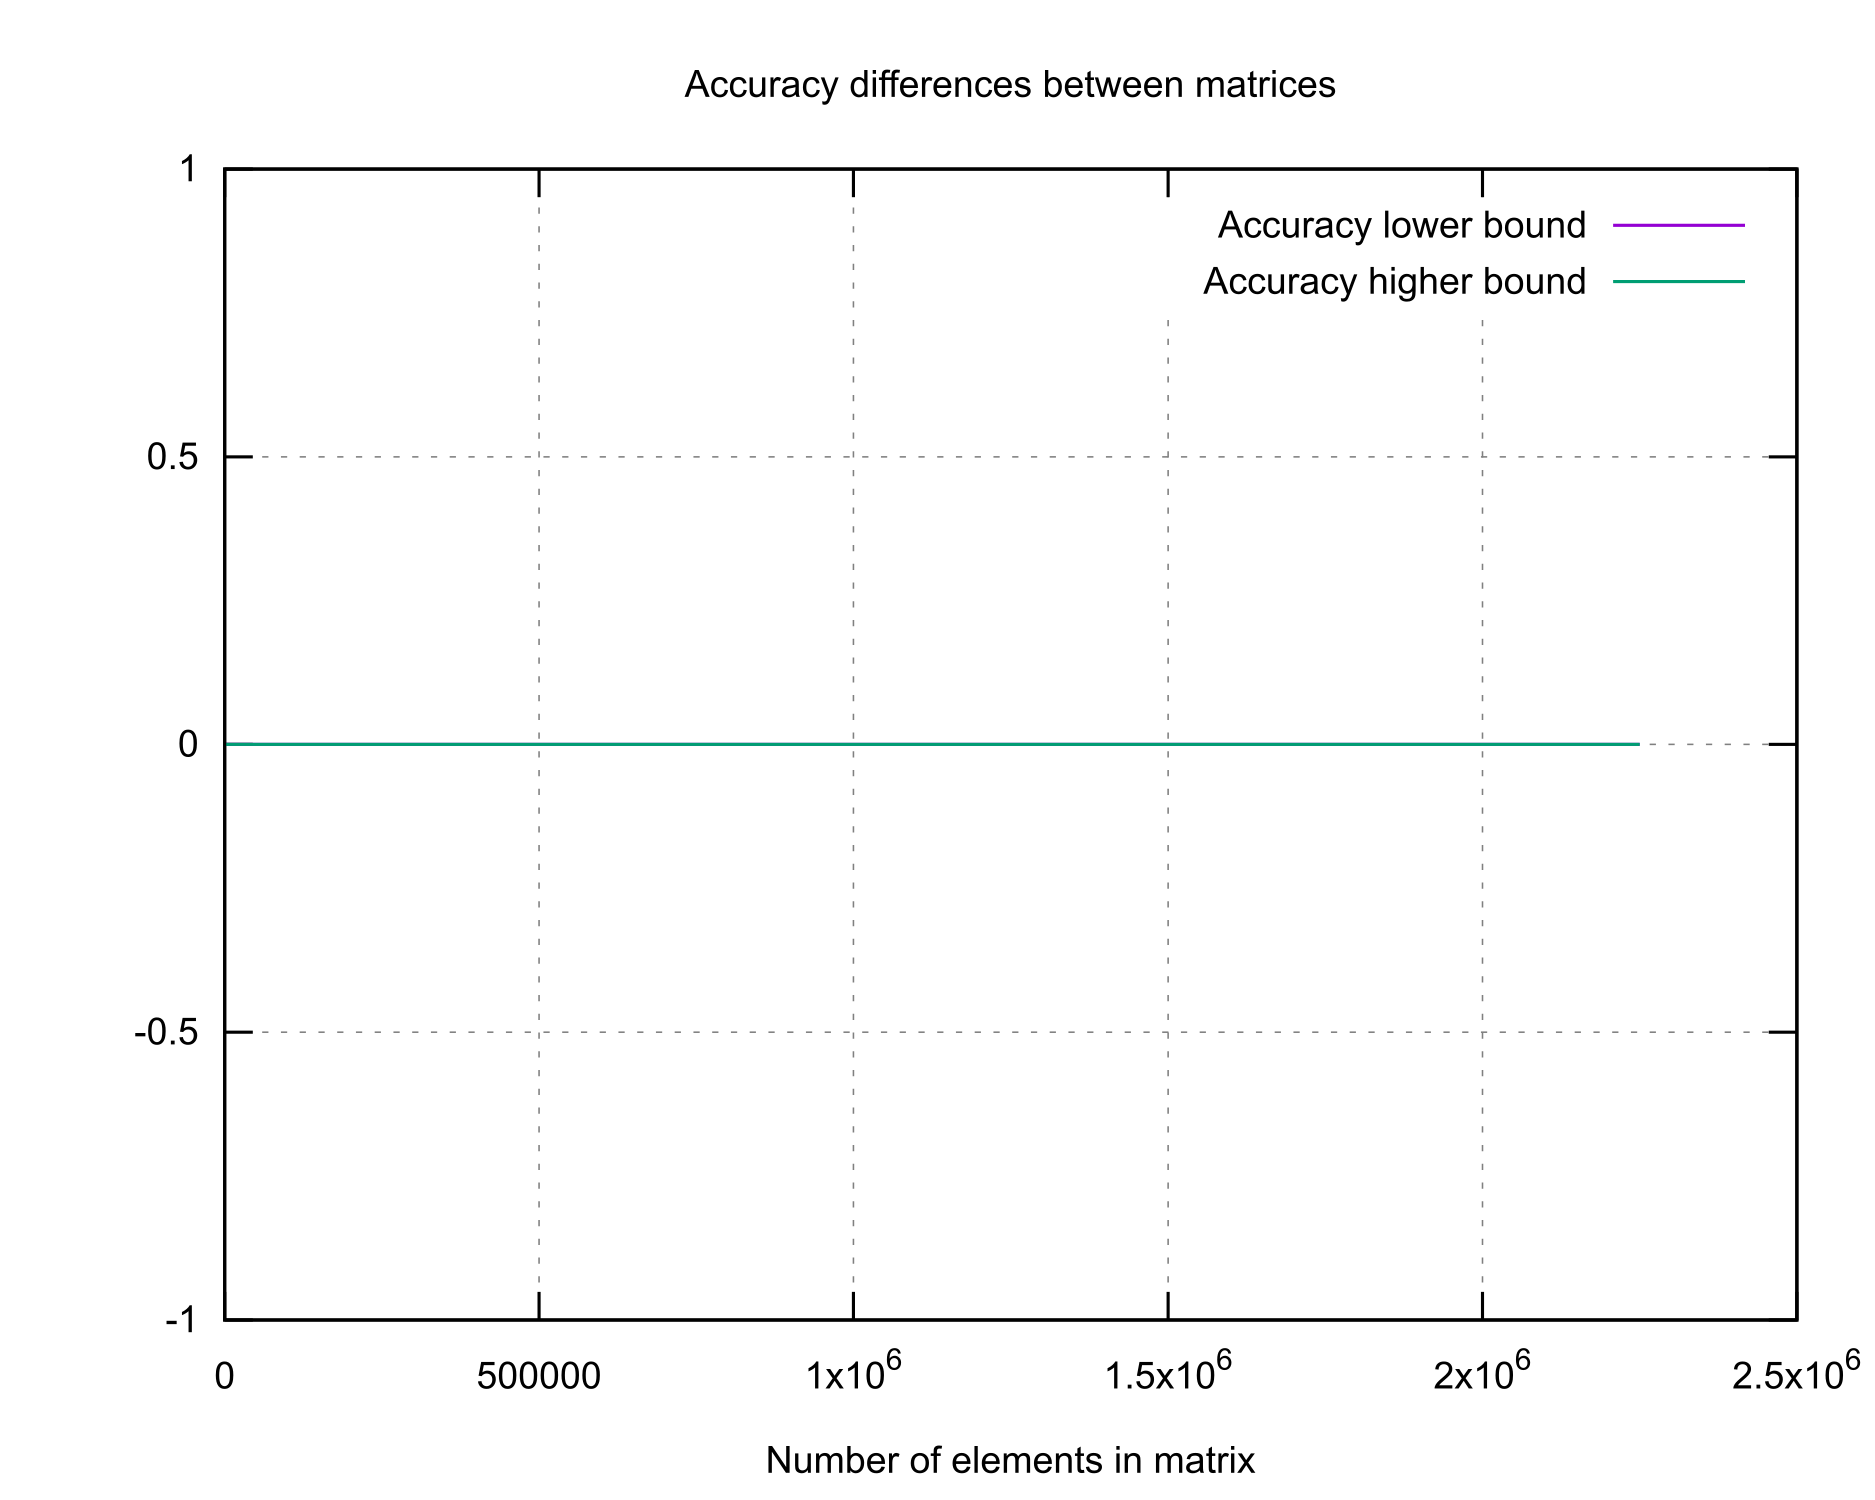
\includegraphics[width=0.6\textwidth]{../../resources/naive_integer_accuracy.png}
    \caption{Écart de précision existant entre les résultats de la méthode Matmult de Numpy 
    et de notre implémentation pour une multiplication sur des \textit{int32}}
    \label{fig:accuracy_naive_integers}
\end{center}
\end{figure}

\subsection{Implémentation non naïve}  

\subsubsection{Idée de l'implémentation}

Cette implementation est tirée du livre \textit{OpenCL Programming Guide}\autocite{openclguide}. 
Son but est de faire usage des \textit{work groups}. Pour cela on fait des tranches de lignes 
dans la matrice afin de les passer à différents \textit{work groups} pour que chaque \textit{work item} 
calcule une ligne de la matrice $C$ (Figure~\ref{fig:non_naive_implementation_principle}). 
\begin{figure}[h]
\begin{center}
    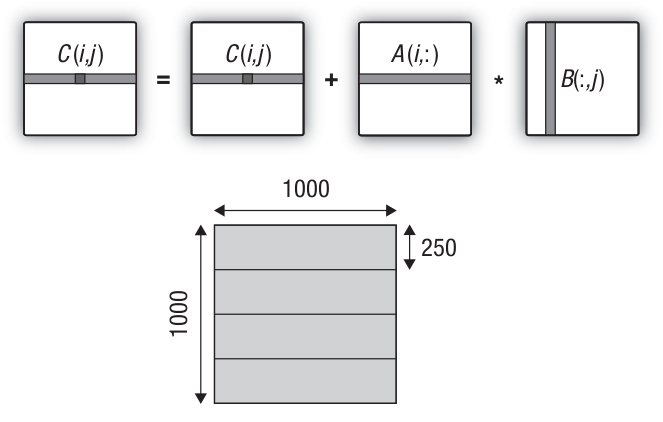
\includegraphics[width=0.6\textwidth]{../../resources/non_naive_implementation_principle.png}
    \caption{Séparation d'une matrice en quatres \textit{work groups}}
    \label{fig:non_naive_implementation_principle}
\end{center}
\end{figure}
De plus, on s'intéresse aux types de mémoire étant donné qu'écrire 
directement dans la mémoire globale causerait des contentions et donc des pertes de performances. 
Les deux autres types de mémoire ici utilisées sont la mémoire locale et la mémoire privée: 
\begin{itemize}
    \item la mémoire locale nous sert à garder les colonnes de la matrice et elle est utilisée par l'ensemble des
        \textit{work items} d'un \textit{work group}
    \item la mémoire privée nous sert à garder les lignes de la matrice car elle n'est utilisée que par un \textit{work
        item}
\end{itemize}
On obtient ainsi le kernel suivant:
\begin{lstlisting}[language=c]
/* #define AWRK_SIZE is added by the host program */
__kernel void matrix_mult(__global float* A,
                          __global float* B,
                          __global float* C,
                          __local float* Bwrk,  /* local memory of b column for work group */
                          const int ncol) {
    int i = get_global_id(0);
    int iloc = get_local_id(0);
    int nloc = get_local_size(0);

    float Awrk[AWRK_SIZE];  /* private memory of a column for work item */

    if (i < ncol) {
        /* copy elements in private memory */
        for (int k = 0 ; k < ncol ; k++) {
            Awrk[k] = A[i * ncol + k];
        }

        for (int j = 0 ; j < ncol ; j++) {
            /* copy elements in local memory */
            for (int k = iloc ; k < ncol ; k = k + nloc) {
                Bwrk[k] = B[k * ncol + j];
            }
            barrier(CLK_LOCAL_MEM_FENCE);
            float tmp = 0.0;
            for (int k = 0 ; k < ncol ; k++) {
                tmp += Awrk[k] * Bwrk[k];
            }
            C[i * ncol + j] = tmp;
        }
    }
}
\end{lstlisting}
\vspace{20pt}

Comme on peut le voir, on passe toujours les matrices par la mémoire globale. 
On définit aussi la mémoire locale \textit{Bwrk} qui est vide au 
départ. En effet, on la remplie à chaque fois que l'on change de colonne en 
itérant sur \textit{j}. On note notamment 
l'utilisation de \textit{barrier\@(CLK\_LOCAL\_MEM\_FENCE)} qui nous permet de 
nous assurer que la mémoire globale a été remplie dans son entiereté avant 
qu'aucun \textit{work item} du \textit{work group} ne commence son calcul. 
Enfin, le remplissage de la mémoire privée se fait en itérant sur la ligne 
de la matrice concernant notre \textit{work item}.

En partant du principe que l’ensemble des éléments pour OpenCL ont été définis (voir Section 3)
et le programme compilé dans la variable program, la mise oeuvre est réalisée de la façon suivante en
Python:
\begin{lstlisting}[language=python]
import numpy as np
import pyopencl as cl

N_WORK_GROUPS = 32
# we keep size which represents a lenght of a line/colunm 
# by powers of two to be able to divide evenly everything for work groups
size = next_power_of_two32bit(max([A_dim[0], A_dim[1], B_dim[0], B_dim[1]]))    

A = np.random.rand(A_dim[0] * A_dim[1]).astype(np.float32)   
B = np.random.rand(B_dim[0] * B_dim[1]).astype(np.float32)   
C = np.zeros(A_dim[1] * B_dim[0], dtype=np.float32)

# our matrices are now of dimensions (size, size)
A = matrix_resize_with_zeros(A, size)
B = matrix_resize_with_zeros(B, size)
C = matrix_resize_with_zeros(C, size)

A_buffer = cl.Buffer(context, flags=cl.mem_flags.READ_ONLY, size=A.nbytes)
B_buffer = cl.Buffer(context, flags=cl.mem_flags.READ_ONLY, size=B.nbytes)
C_buffer = cl.Buffer(context, flags=cl.mem_flags.WRITE_ONLY, size=C.nbytes)

cl.enqueue_copy(queue, src=A, dest=A_buffer)
cl.enqueue_copy(queue, src=B, dest=B_buffer)

kernel_arguments = (A_buffer, B_buffer, C_buffer,
                    # local memory size needs to be passed for
                    # local argument
                    cl.LocalMemory(A[0].nbytes),
                    np.int32(size))
start = time.time()
program.matrix_mult(queue,
                    [size],
                    [size // N_WORK_GROUPS],
                    *kernel_arguments).wait()

cl.enqueue_copy(queue, src=C_buffer, dest=C)

matrices_resize_original_dimensions(C, A_dim[0], B_dim[1])
\end{lstlisting}
\vspace{20pt}

On remarque déjà qu'on a fait du \textit{padding} pour rendre nos matrices 
carrés. Ceci permet de nous assurer qu'il n'y aura pas de problème lors de 
la répartition des \textit{work groups}. On rappelle en effet qu'il faut que
$size \bmod N\_WORK\_GROUPS = 0$. On note aussi que l'on doit passer 
un object du type \textit{pyopencl.LocalMemory} en paramètre afin de pouvoir 
demander à \texttt{OpenCL} d'allouer tant d'octets à la mémoire locale de chaque
\textit{work group}.

\subsubsection{Résultats}

On a fait trois genres de mesures afin de voir l'éfficacité et la fiabilité 
de l'implémentation: la copie des \textit{buffers}, le temps d'exécution et 
la précision des résultats. Pour faire ces mesures on a exécuté le programme 
pour des matrices carrées de même dimension allant de 10 à 1 500 lignes/colonnes par pas de 10. 
Tous les graphes peuvent êtres retrouvées avec une meilleure résolution en annexe.
On verra que ces derniers ne sont pas concluants malgré le fait que ce soit une implémentation 
optimisée\autocite{openclguide}.


\begin{figure}[H]
\begin{center}
    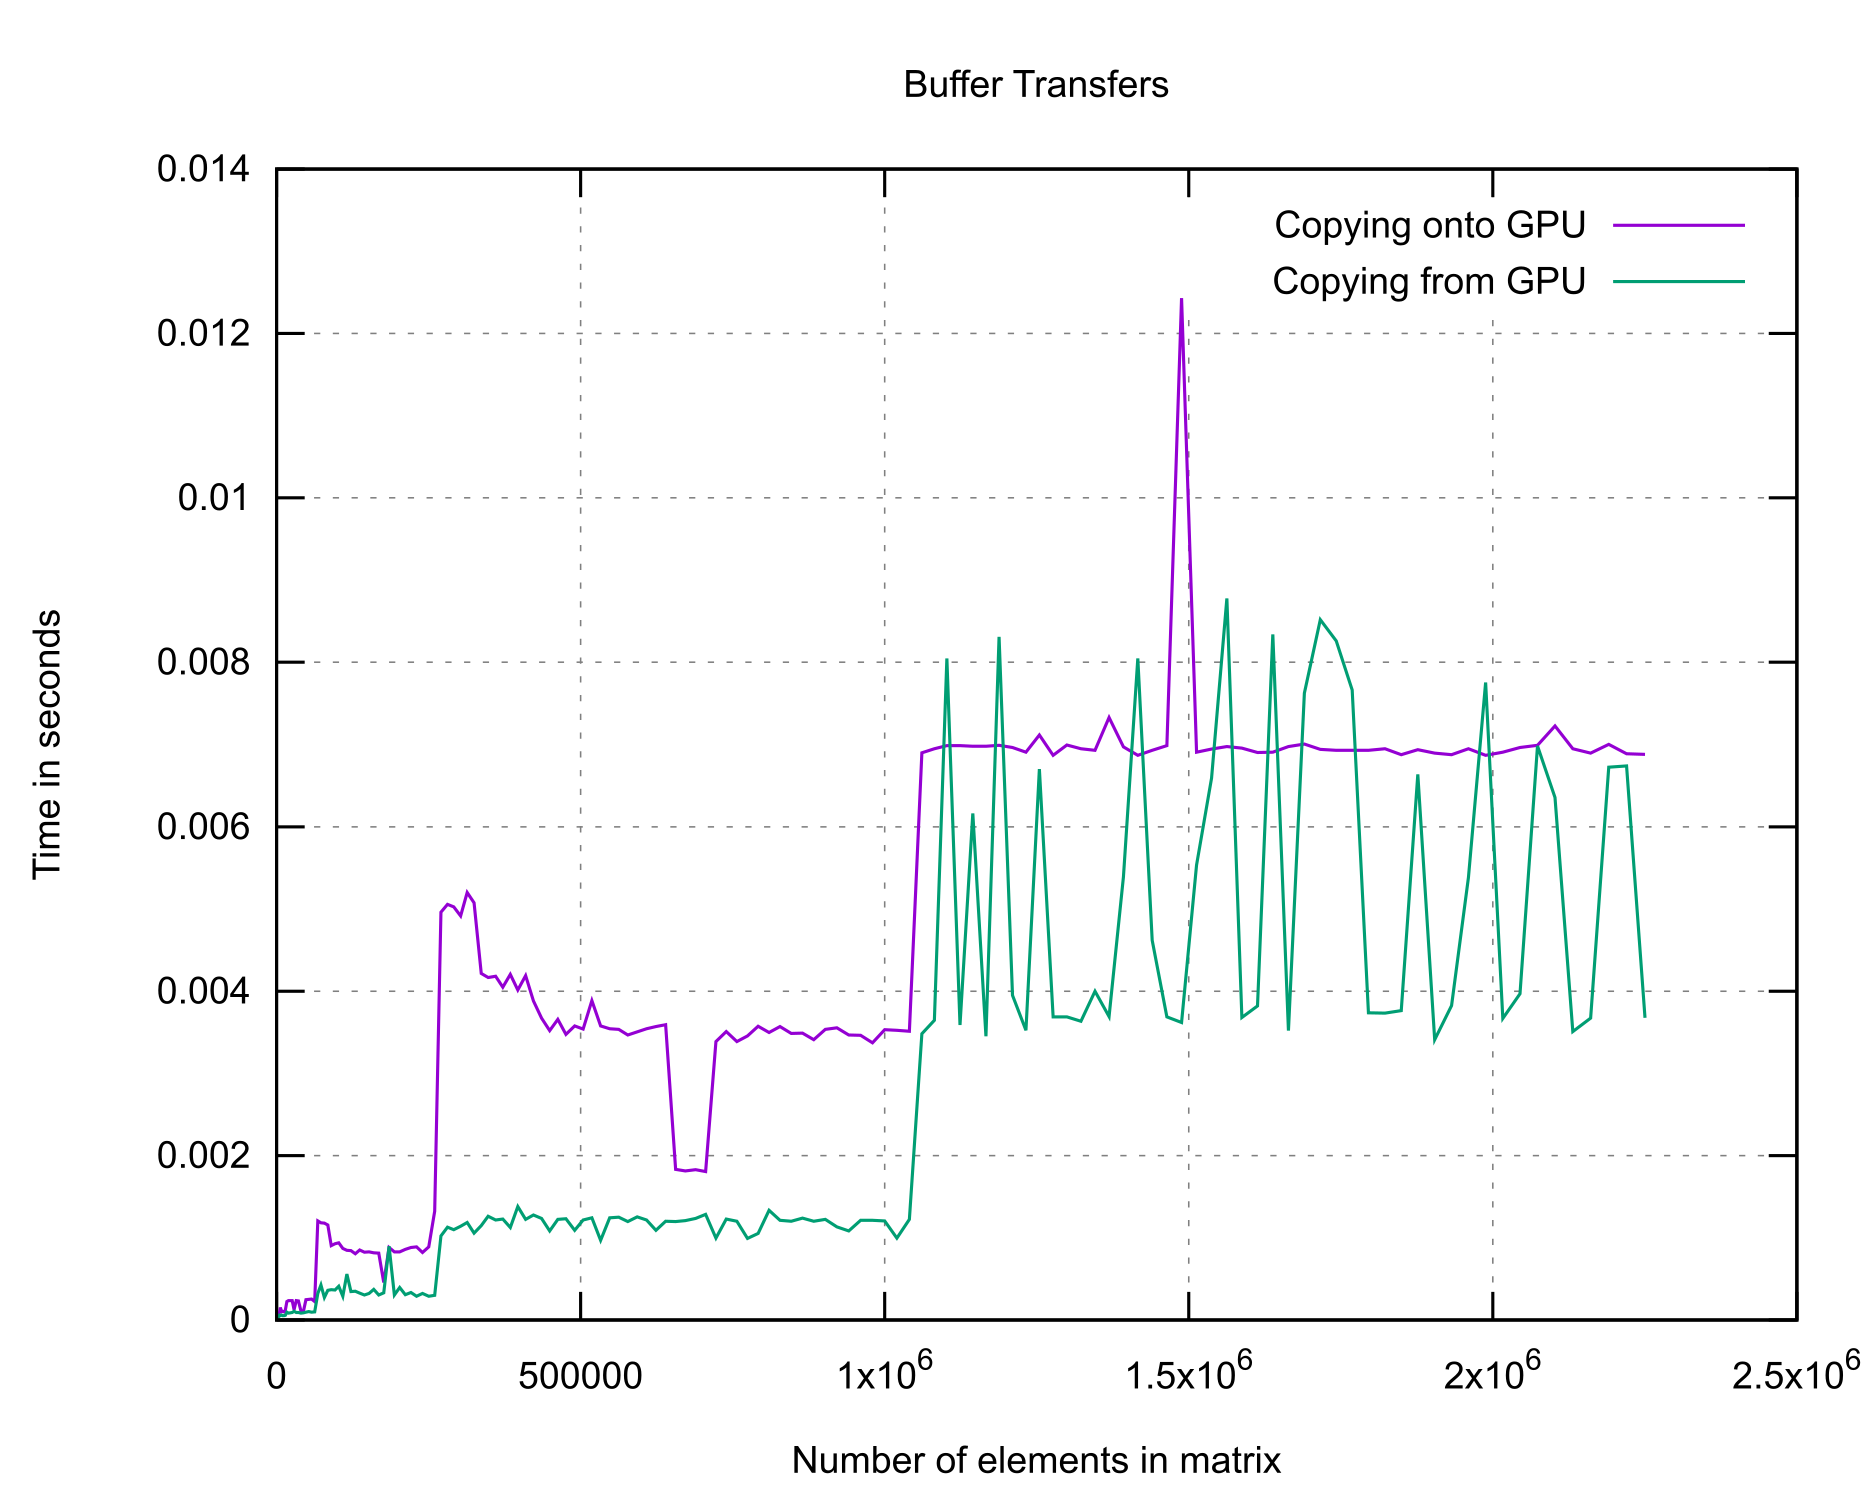
\includegraphics[width=0.6\textwidth]{../../resources/buffer_transfer.png}
    \caption{Temps de copie des \textit{buffers} de \textit{float32} entre l'hôte et le GPU}
    \label{fig:buffer_transfer}
\end{center}
\end{figure}

La copie des buffers bouge par palier comme on peut le voir
(Figure~\ref{fig:buffer_transfer}). Ceci est du au \textit{padding} étant 
donné qu'un matrice de dimension (1000, 1000) par exemple sera ramené à une dimension 
de (1024, 1024). On n'explique cependant pas l'irrégularité que l'on peut observer.

\begin{figure}[H]
\begin{center}
    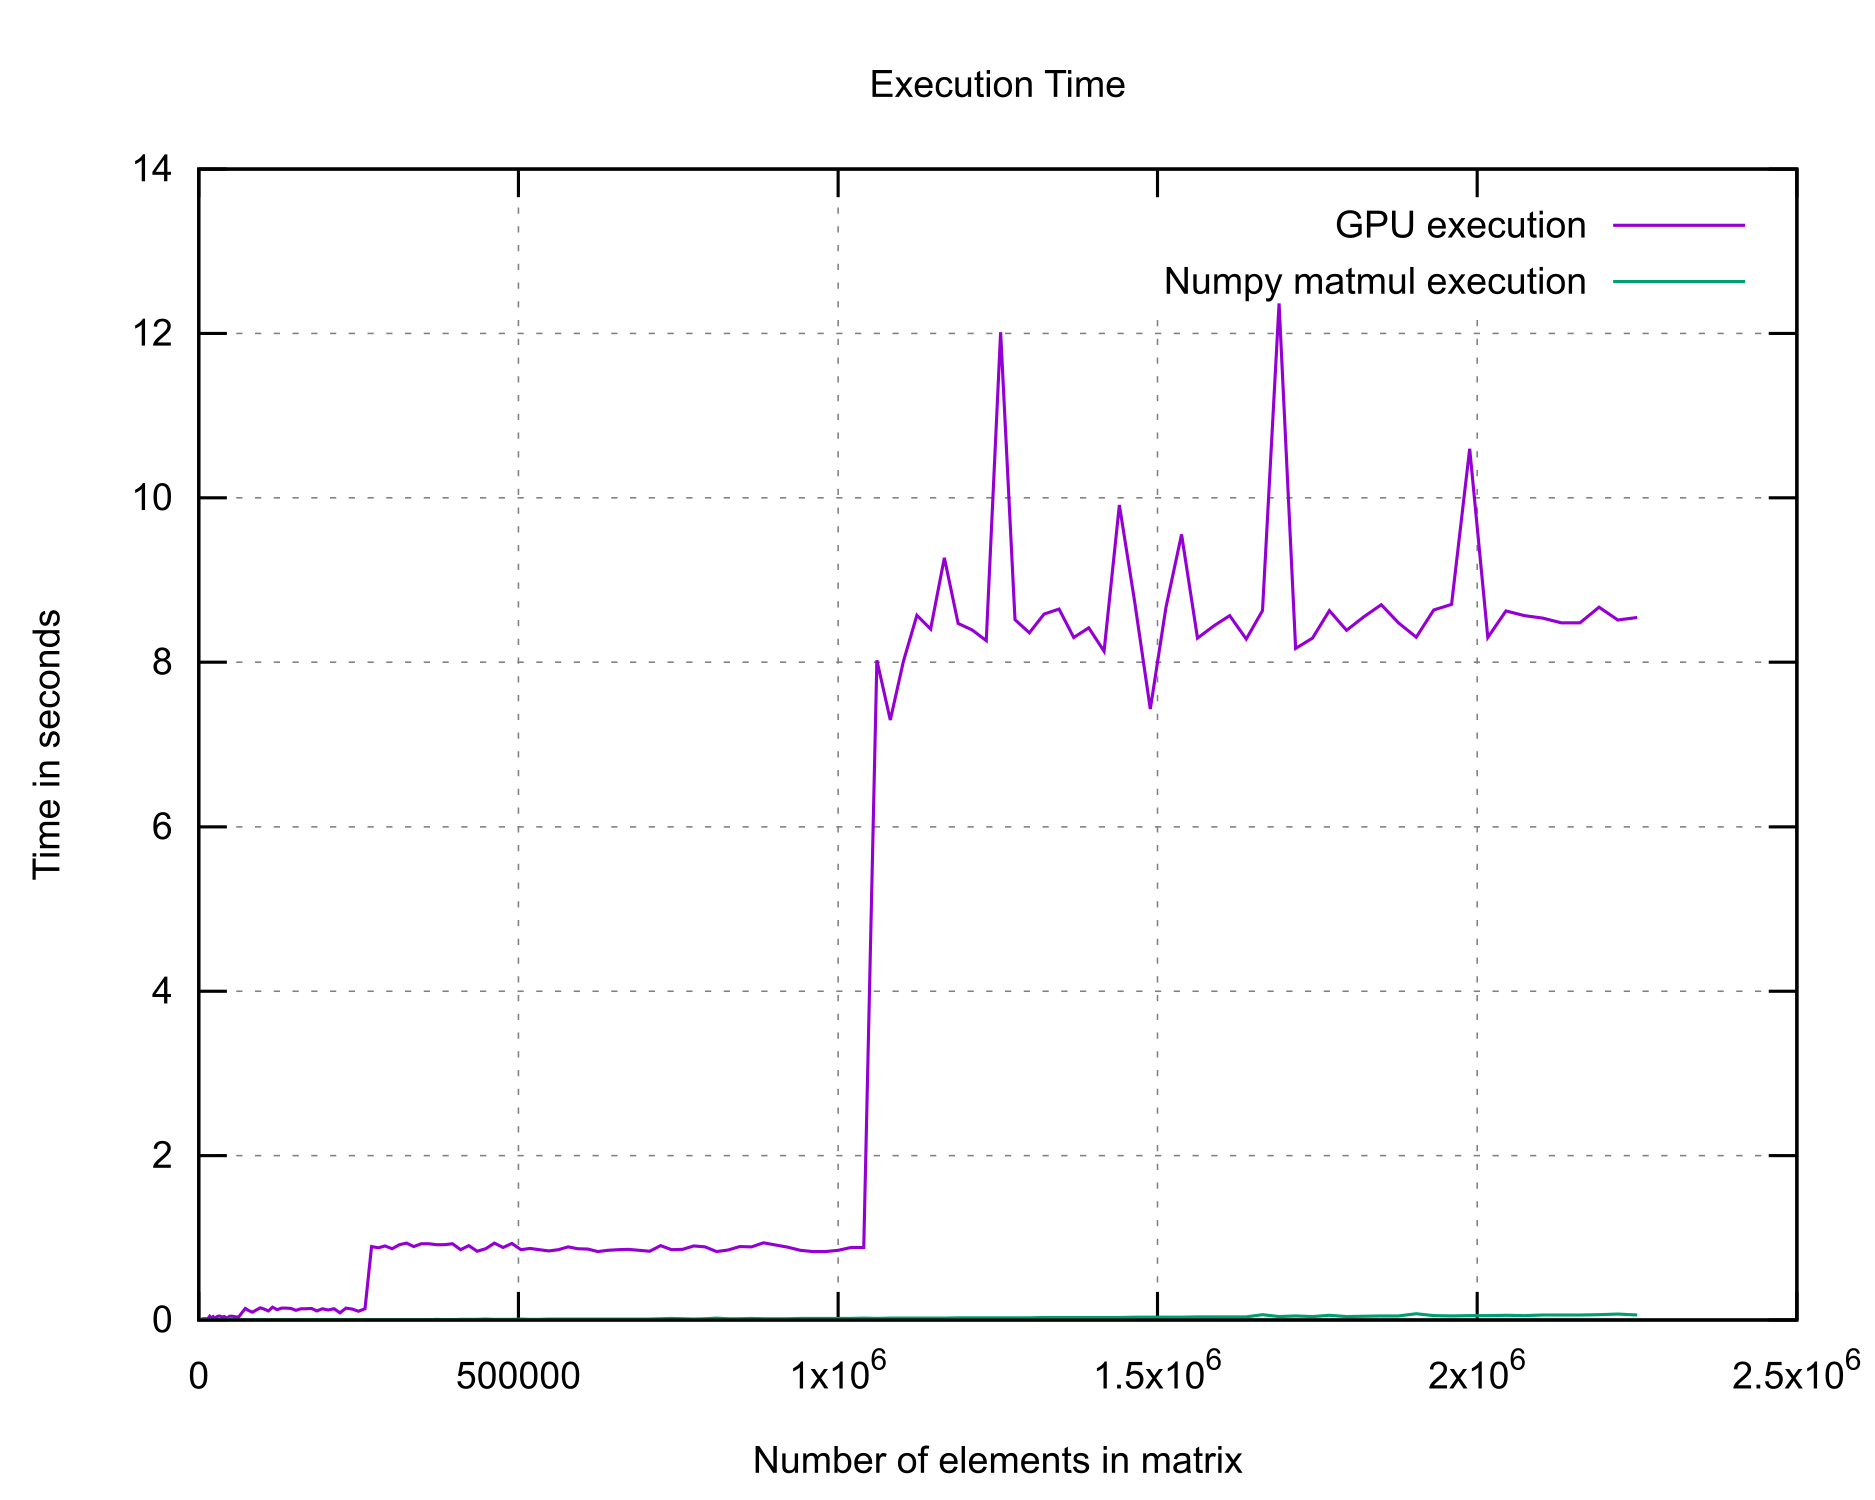
\includegraphics[width=0.6\textwidth]{../../resources/execution_time.png}
    \caption{Temps d'exécution de notre implémentation et de la méthode Matmult de \texttt{Numpy}
    pour une multiplication sur des \textit{float32}}
    \label{fig:execution_time}
\end{center}
\end{figure}

Le temps d'exécution de notre implémentation monte lui aussi par pallier comme attendu
(Figure~\ref{fig:execution_time}). On note cependant que notre implémentation 
est beaucoup plus lente que celle de \texttt{Numpy} et aussi que l'implémentation naïve. 
On ne l'explique pas.

\begin{figure}[H]
\begin{center}
    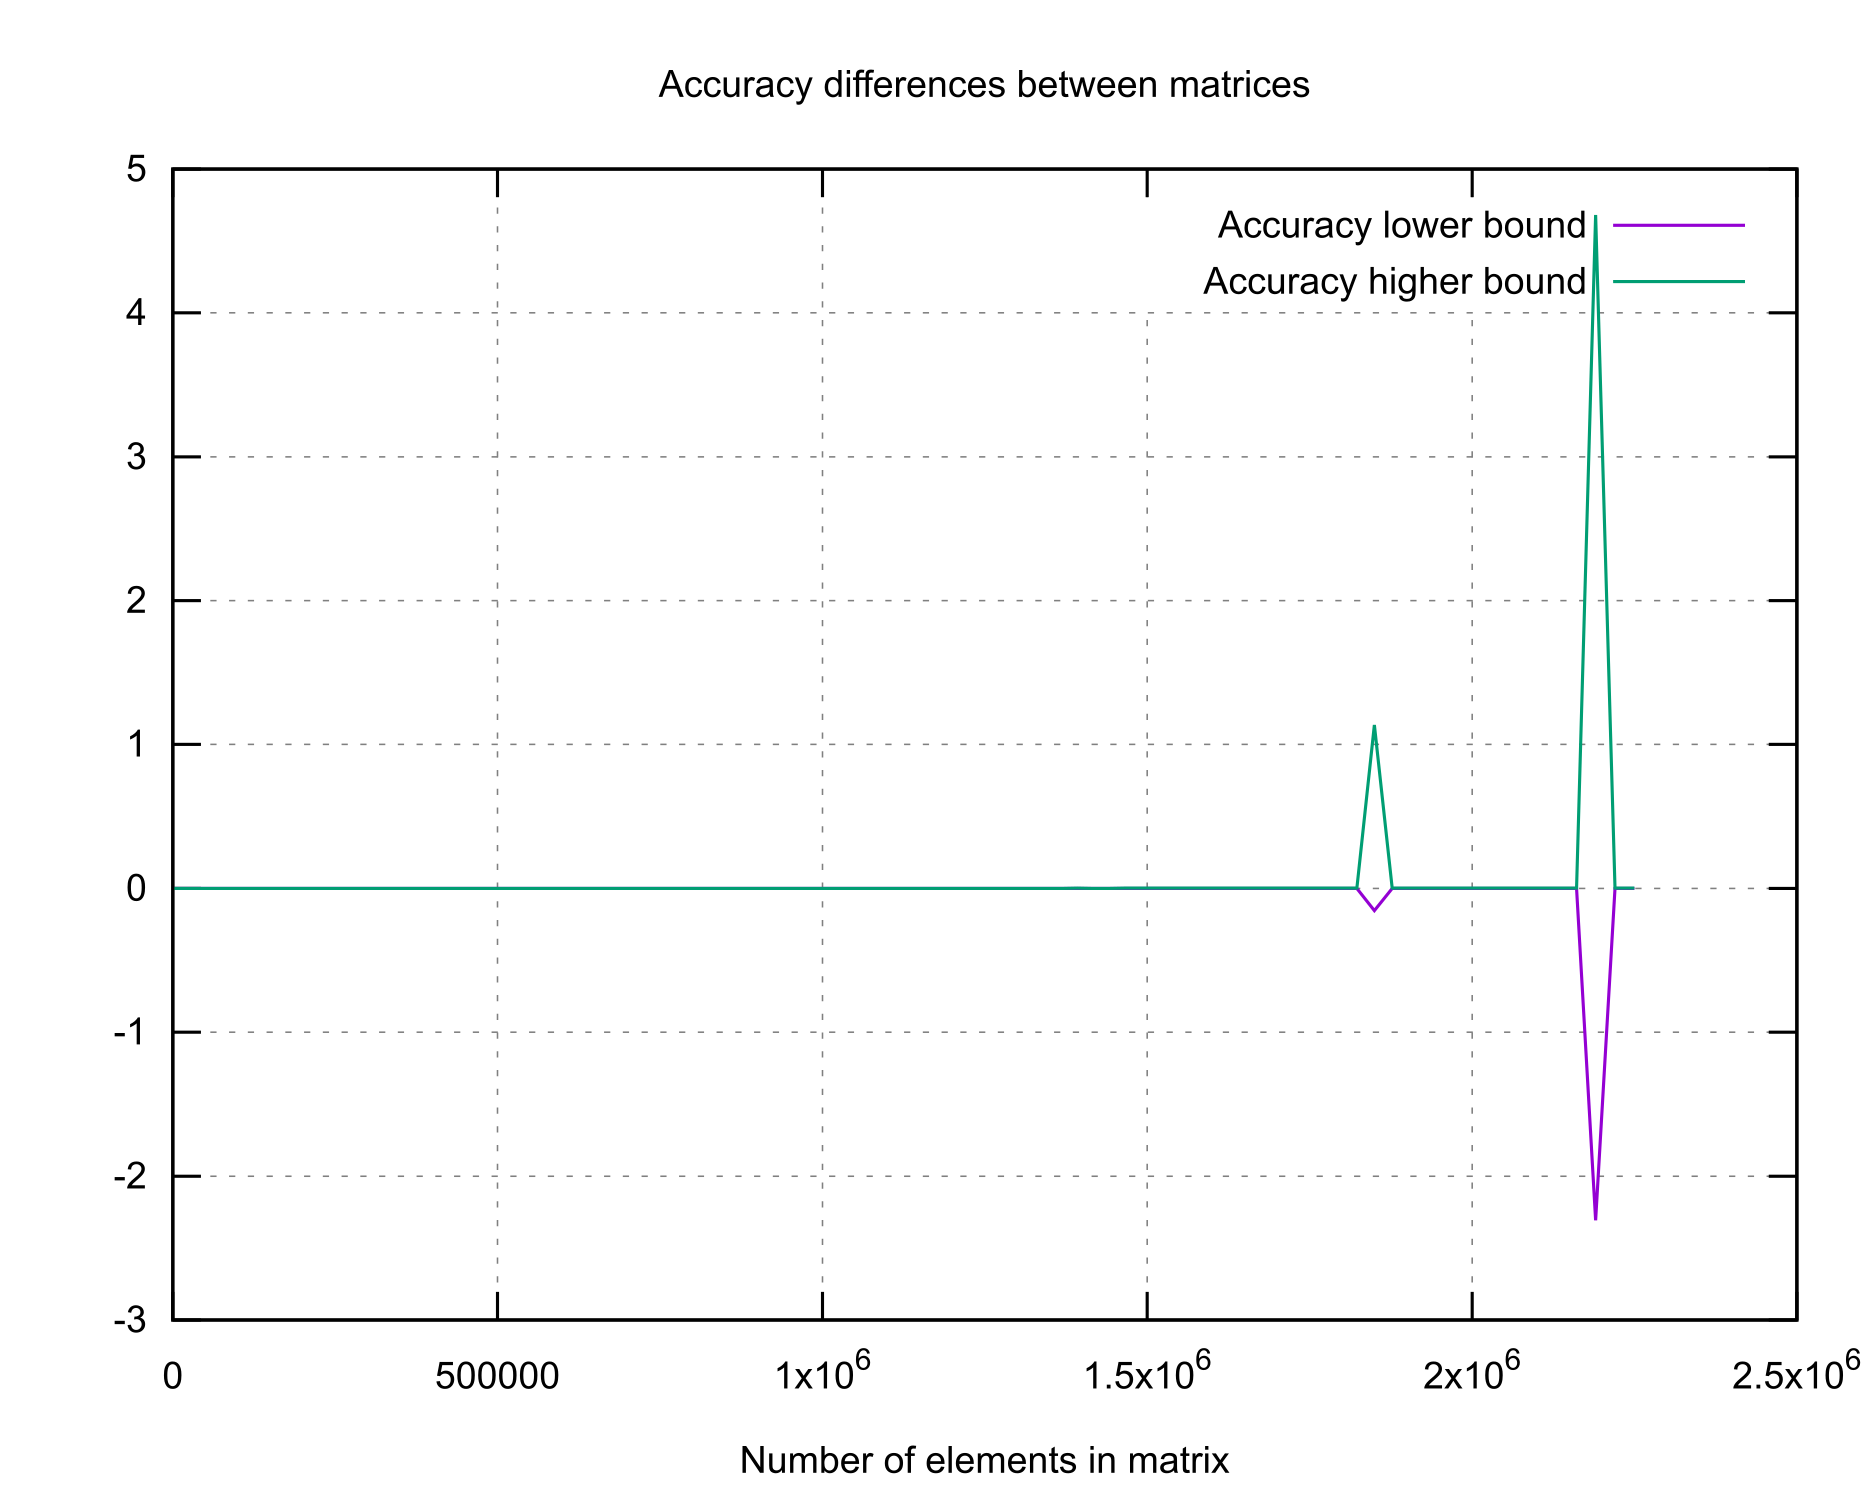
\includegraphics[width=0.6\textwidth]{../../resources/float_accuracy.png}
    \caption{Écart de précision existant entre les résultats de la méthode Matmult de Numpy 
    et de notre implémentation pour une multiplication sur des \textit{float32}}
    \label{fig:accuracy}
\end{center}
\end{figure}

Enfin, on constate moins d'écart entre les éléments des matrices résultantes de \texttt{Numpy} et 
de notre implémentation (Figure~\ref{fig:accuracy}). Cependant, certains pics d'écarts sont visibles. 
Ici non plus, on ne l'explique pas.

Cette partie est une incompréhension totale car cette implémentation nous est vendue comme 
une implémentation optimisée. On se demande si ce n'est pas parce qu'elle ne serait pas 
trop adapté au du matériel utilisé. Mais on l'a tout de même pris en considération, par exemple: 
l'utilisation de 32 \textit{work groups} n'est pas aléatoire, c'est parce qu'on a 32 
\textit{compute units} sur notre GPU\@. De ce fait, il aurait été intéressant de pouvoir tourner cette 
implémentation sur un autre GPU de manière à pouvoir comprendre si c'est ce dernier qui 
est à la cause de celà.
